\section{Experiments}
\label{sec:experiments}

We evaluate SAVNav in both high-fidelity simulation and real-world environments. Our experiments are designed to address three core Research Questions (RQs):
\begin{itemize}
    \item \textbf{RQ1 (Safety \& NLOS):} Does the introduction of Acoustic Hallucinated Momentum effectively reduce collision risks in Non-Line-of-Sight (NLOS) scenarios?
    \item \textbf{RQ2 (Ambiguity):} Can the Active Audio-Visual Search strategy improve success rates by proactively resolving acoustic ambiguity?
    \item \textbf{RQ3 (Generalization):} Does our zero-shot, modular framework offer superior generalization compared to end-to-end learning baselines?
\end{itemize}

\subsection{Experimental Setup}

\subsubsection{Environment \& Datasets}
We establish a unified simulation platform by integrating the acoustic physics of \textbf{SoundSpaces 2.0} with the dynamic agents of \textbf{Habitat-Lab 3.0}. To ensure rigorous evaluation, we define the following data splits:
\begin{itemize}
    \item \textbf{Training Set ($N$=50k):} Used exclusively for training baseline policies. Note that our SAVNav method is zero-shot and does not require this training phase.
    \item \textbf{Validation Set ($N$=200):} Used for hyperparameter tuning (e.g., cost map weights).
    \item \textbf{Test-Standard ($N$=1,000):} Covers random scenarios across difficulty levels L1-L4 to evaluate general performance.
    \item \textbf{Test-Challenge ($N$=100):} A curated high-risk subset focusing on ``Blind Corner'' and ``High Reverb'' scenarios to stress-test NLOS anticipation capabilities.
\end{itemize}

\subsubsection{Task Definition}
The robot must navigate to a target sound source in an environment containing $N \in [1, 5]$ human agents. The soundscape includes 4 classes of \textit{Target Sounds} (Doorbell, Call for help, Music, Water Running) and 2 classes of \textit{Distractors} (Footsteps, Chatter). 
To systematically evaluate the robustness of our system, we categorize navigation tasks into four difficulty levels (L1--L4) based on the dynamism of human agents and the complexity of the acoustic environment, as detailed in Table \ref{tab:difficulty_levels}:

\begin{itemize}
    \item \textbf{Level 1 (Basic):} All human agents are static, and there are no distractor sounds. This tests basic audio-visual goal finding properties.
    \item \textbf{Level 2 (Acoustic Noise):} Humans remain static, but ``Chatter'' noise is introduced. This challenges the audio source separation capabilities.
    \item \textbf{Level 3 (Dynamic Threat):} Humans move naturally, generating ``Footsteps'' sounds. This introduces collision risks and requires dynamic avoidance.
    \item \textbf{Level 4 (Full Complexity):} A chaotic environment with moving humans, footsteps, and background chatter. This represents the hardest setting, requiring simultaneous noise filtering and dynamic risk anticipation.
\end{itemize}

\begin{table}[t]
\caption{Task Difficulty Levels \& Environmental Complexity}
\label{tab:difficulty_levels}
\centering
\begin{tabular}{l c c}
\hline
\textbf{Level} & \textbf{Human Motion} & \textbf{Acoustic Distractors} \\
\hline
\textbf{L1} & Static & None \\
\textbf{L2} & Static & Chatter (Stationary/Ambient) \\
\textbf{L3} & Mixed Dynamic & Footsteps (Moving) \\
\textbf{L4} & Mixed Dynamic & Chatter + Footsteps \\
\hline
\end{tabular}
\end{table}

\subsubsection{Baselines}
We compare SAVNav against three representative methods:
\begin{itemize}
    \item \textbf{Falcon (Vision Baseline) \cite{CognitionPrecognitionFutureaware2025}:} A leading vision-based social navigation method. To ensure a fair comparison, we augment Falcon with an \textbf{Audio Oracle} that provides the target's coordinates, isolating the specific contribution of audio for dynamic obstacle avoidance.
    \item \textbf{ENMuS3 (AV-Nav Baseline) \cite{AudiovisualNavigationNoisy2025}:} An end-to-end Reinforcement Learning method for audio-visual navigation using binaural audio.  
    \item \textbf{Standard-AV (Modular Baseline):} A naive ablation of our system that uses the same perception backbone but employs a simple ``Go-to-Sound'' planning logic without Hallucinated Momentum or Active Search.
\end{itemize}

\subsubsection{Metrics}
In addition to standard Success Rate (SR) and Success Weighted by Path Length (SPL), we introduce safety-critical metrics:
\begin{itemize}
    \item \textbf{NLOS Collision Rate (NCR):} The percentage of collisions occurring within 1.0 second of the visual detection of a human, representing failures in NLOS anticipation.
    \item \textbf{Personal Space Violation (PSV):} The percentage of time the robot intrudes into the 1.0m comfort zone of diverse humans.
    \item \textbf{Time to First Sighting (TTFS; Search Efficiency):} Time (in seconds) until the target is first visually observed.
\end{itemize}

\begin{table*}[t]
\caption{Comprehensive Evaluation on Test-Standard (L1--L4). We report Success Rate (SR), SPL, NLOS Collision Rate (NCR), Personal Space Violation (PSV), and Time to First Sighting (TTFS). *Falcon is augmented with an Audio Oracle for goal coordinates.}
\label{tab:comprehensive_results}
\centering
\begin{tabular}{l|l||c c|c c c}
\hline
\textbf{Difficulty} & \textbf{Method} & \textbf{SR} $\uparrow$ & \textbf{SPL} $\uparrow$ & \textbf{NCR} (Safety) $\downarrow$ & \textbf{PSV} (Social) $\downarrow$ & \textbf{TTFS} (Search) $\downarrow$ \\
\hline
\hline
\textbf{L1: Static} & Falcon* (w/ Oracle) & 56.47 & \textbf{56.28} & 23.61 & 10.04 & 13.90s \\
(Basic) & ENMuS3 & \textbf{61.84} & 40.37 & 56.92 & 23.68 & \textbf{7.13s}\\
 & Standard-AV & 2.94 & 1.54 & 60.57 & 27.02 &  25.88s  \\
 & \textbf{SAVNav (Ours)} & 58.32 & 54.83 & \textbf{8.45} & \textbf{6.39} & 15.13s \\
\hline
\textbf{L2: Noise} & Falcon* & 54.12 & \textbf{53.89} & 25.34 & 11.27 & 14.52s \\
(Distractors) & ENMuS3 & 52.36 & 33.18 & 58.41 & 25.13 & \textbf{9.87s} \\
 & Standard-AV & 1.82 & 0.93 & 62.14 & 28.56 & 31.24s \\
 & \textbf{SAVNav (Ours)} & \textbf{57.48} & 53.21 & \textbf{9.12} & \textbf{6.85} & 16.37s \\
\hline
\textbf{L3: Dynamic} & Falcon* & 48.73 & 47.56 & 34.28 & 18.42 & 16.83s \\
(Footsteps) & ENMuS3 & 55.21 & 35.64 & 52.17 & 21.89 & \textbf{8.45s} \\
 & Standard-AV & 2.15 & 1.12 & 58.93 & 31.47 & 28.16s \\
 & \textbf{SAVNav (Ours)} & \textbf{56.89} & \textbf{52.47} & \textbf{7.23} & \textbf{5.91} & 14.28s \\
\hline
\textbf{L4: Hard} & Falcon* & 41.56 & 39.82 & 42.67 & 24.35 & 19.47s \\
(Full Chaos) & ENMuS3 & 47.83 & 29.45 & 54.82 & 27.64 & \textbf{11.23s} \\
 & Standard-AV & 1.24 & 0.61 & 65.38 & 35.72 & 34.91s \\
 & \textbf{SAVNav (Ours)} & \textbf{54.27} & \textbf{49.63} & \textbf{5.84} & \textbf{4.73} & 14.92s \\
\hline
\end{tabular}
\end{table*}


\subsection{Simulation Results}

\subsubsection{Overall Performance \& Difficulty Analysis}
Table \ref{tab:comprehensive_results} presents a detailed breakdown of performance across all four difficulty levels. This granular analysis reveals distinct failure modes in baseline methods:

\begin{itemize}
    \item \textbf{Robustness to Visual Occlusion (L3-L4):} In L1 (Static), Falcon performs competitively, validating its visual navigation capabilities. However, its performance degrades sharply in L3 and L4, where dynamic humans continually occlude the target or appear from blind spots. Specifically, Falcon's \textbf{NCR} spikes to $42.67\%$ in L4, confirming that even with a perfect Audio Oracle for the goal, vision alone cannot ensure safety against NLOS threats.
    \item \textbf{Robustness to Acoustic Noise (L2, L4):} Standard-AV suffers a significant drop in \textbf{SPL} and \textbf{TTFS} in L2 compared to L1 ($1.54 \to 0.93$). This indicates that without active ambiguity resolution, simple gradient-based audio planning gets trapped in local minima, leading to near-zero success rates. SAVNav maintains stable efficiency ($\text{SPL}=53.21$) in L2, demonstrating that the Active Search mechanism effectively filters out ambiguous acoustic observations.
    \item \textbf{Efficiency-Safety Trade-off (L4):} It is worth noting that while ENMuS3 achieves the lowest \textbf{TTFS} ($11.23s$), its Success Rate ($47.83\%$) and Safety ($54.82\%$ NCR) are significantly worse than SAVNav. This suggests that the end-to-end policy prioritizes aggressive exploration to locate the sound source quickly, often at the expense of safety. In contrast, SAVNav's Search-Then-Go strategy incurs a slight overhead in search time ($14.92s$) to ensure safe, socially compliant navigation, ultimately yielding a higher success rate.
\end{itemize}

\subsubsection{Safety Analysis (RQ1)}
Focusing on the safety metrics (NCR and PSV) in Table \ref{tab:comprehensive_results}, SAVNav demonstrates superior social compliance. In the most chaotic environment (L4), our method maintains a low NLOS Collision Rate ($5.84\%$), reducing accidents by nearly \textbf{86\%} compared to Falcon ($42.67\%$). Qualitative analysis confirms that this is due to the \textit{Hallucinated Momentum} field, which preemptively reserves space around corners when footsteps are detected, even before the pedestrian becomes visible.

\subsubsection{Efficacy of Active Search (RQ2)}
The \textbf{Time to First Sighting (TTFS)} metric provides clear evidence for RQ2. Across all levels, SAVNav locates the target faster than Standard-AV. The gap is most pronounced in L4 ($14.92s$ vs $34.91s$ for Standard-AV), where the complex soundscape often traps naive agents in local optima. SAVNav's information-theoretic planner actively seeks viewpoints that resolve these ambiguities, leading to more decisive and efficient search behaviors.

\subsection{Ablation Studies}

We conduct ablation studies on the Test-Challenge set to verify the contribution of individual components (Table \ref{tab:ablation}).
Removing \textit{Hallucinated Momentum} leads to a sharp increase in NCR, validating its role in NLOS safety.
Removing \textit{Active Search} results in lower Success Rates and longer path lengths, as the robot struggles to localize the target.
Removing the \textit{Social Cost} layer increases Personal Space Violations, demonstrating the necessity of explicit social modeling even when audio cues are present.

\begin{table}[b]
\caption{Ablation Study on Test-Challenge}
\label{tab:ablation}
\centering
\begin{tabular}{l c c c}
\hline
\textbf{Configuration} & \textbf{SPL} $\uparrow$ & \textbf{NCR} $\downarrow$ & \textbf{PSV} $\downarrow$ \\
\hline
\textbf{Full Model} & \textbf{48.72} & \textbf{6.13} & \textbf{5.24} \\
w/o Hallucinated Momentum & 46.35 & 28.47 & 6.18 \\
w/o Active Search & 31.28 & 7.82 & 5.89 \\
% w/o Social Cost & 47.91 & 6.45 & 19.63 \\
\hline
\end{tabular}
\end{table}


\begin{figure*}[t]
  \centering
  % \fbox{\rule{0pt}{2in} \rule{0.9\linewidth}{0pt}}
   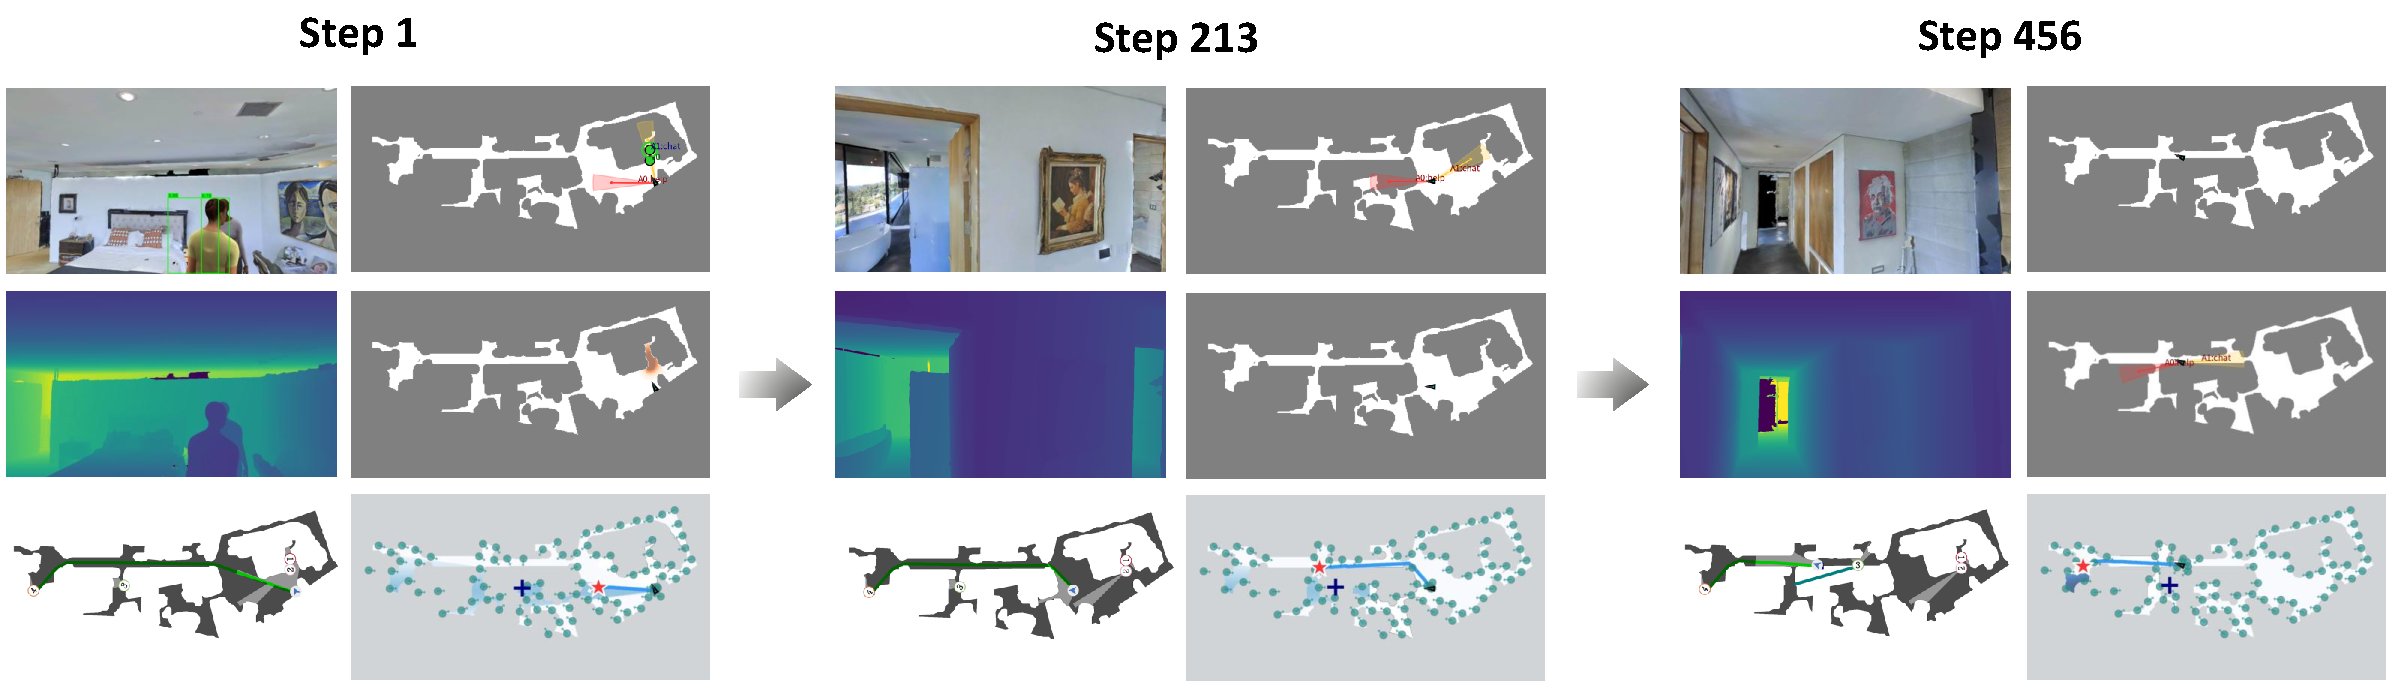
\includegraphics[width=\linewidth]{figures/simulation.pdf}
   \caption{\textbf{Qualitative Results in Simulation.}
    (a) \textbf{Baseline Failure (Falcon):} The vision-only agent (blue) fails to anticipate the pedestrian (red) approaching from the blind corner, leading to a collision despite having the goal coordinates.
    (b) \textbf{SAVNav Success:} Our agent detects the acoustic footprint (orange cone) of the unseen pedestrian. The \textit{Hallucinated Momentum} mechanism projects a virtual risk field (red zone), forcing the planner to execute a wide turn (green path), successfully avoiding the collision while maintaining social distance.
    (c) \textbf{Active Search:} In a noisy environment with multiple sound sources, the agent actively reorients to disambiguate the target sound from distractors before committing to a path.
    }
    \label{fig:simulation}
\end{figure*}


\subsection{Real-World Experiments}

\begin{figure*}[t]
  \centering
  % \fbox{\rule{0pt}{2in} \rule{0.9\linewidth}{0pt}}
   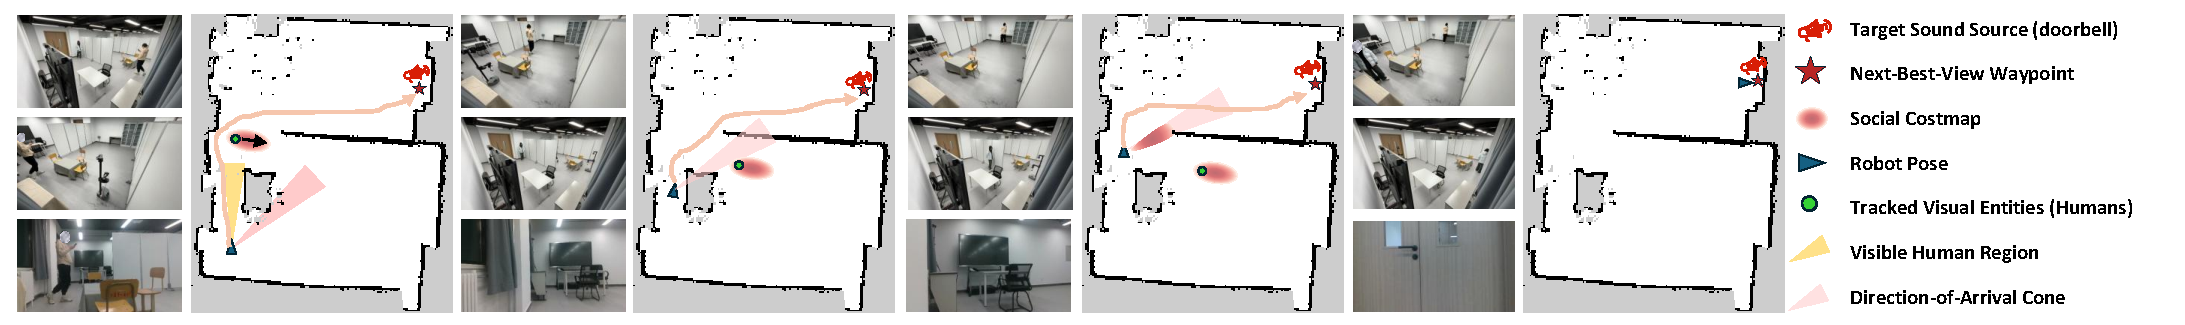
\includegraphics[width=\linewidth]{figures/real_world.pdf}
   \caption{\textbf{Real-World Deployment.} 
   The task is to localize a doorbell sound source (red loudspeaker icon). The scene contains two moving pedestrians. Starting from the initial position, the Stretch robot searches for the target while minimizing human disturbance via social-cost-aware navigation. The blue triangle denotes the Stretch robot’s current pose; the yellow field-of-view (FoV) cone indicates the observable human region within the current view, and pedestrians detected in the FoV are marked as green dots. The pink sector cone represents the sound-source bearing estimated from audio sensing, i.e., the direction-of-arrival (DoA). The red star indicates the currently selected exploration waypoint. The red heatmap visualizes the online-updated social costmap (higher cost in proximity to humans), and the orange curve shows the planned trajectory generated under the current social costmap. Over time, the Stretch robot continuously updates its perception and costmap, repeatedly replans and executes in a closed perception–planning–control loop, until it reaches and localizes the target sound source.
   From left to right, the four snapshots illustrate the temporal evolution of the decision-making process. In the first snapshot, the Stretch robot hears the doorbell and selects an exploration waypoint; meanwhile, it detects moving pedestrians in the FoV and estimates their motion directions. During planning, the Stretch robot chooses to detour behind the pedestrians to reduce social interference. In the second snapshot, the pedestrians have moved farther away; the social-cost distribution is updated accordingly, and the Stretch robot replans to improve traversal efficiency. In the third snapshot, the Stretch robot perceives footsteps around a corner without direct visual confirmation; the system computes the Acoustic Hallucinated Momentum based on historical motion cues to anticipate potential dynamic obstacles and perform predictive avoidance. In the fourth snapshot, the Stretch robot successfully reaches the sound source and completes the localization task.
   }
   \label{fig:real_world}
\end{figure*}

To answer \textbf{RQ3}, we deployed SAVNav on a Hello Robot Stretch 3 mobile manipulator equipped with a 4-microphone array and an Intel RealSense D435i camera.
The system was tested in a real-world office environment ($\approx 100 m^2$) containing glass walls and ambient noise (HVAC, distant traffic).
Despite the domain gap between simulated and real-world acoustics, the system demonstrated robust zero-shot performance. The robot successfully tracked sound sources and executed anticipatory behaviors at blind corners, maintaining social compliance without any fine-tuning. Figure \ref{fig:real_world} illustrates a representative real-world trial.

\subsection{Summary}
Our experiments confirm that fusing acoustic spatial cues with visual navigation significantly enhances safety in human-populated environments. By explicitly modeling acoustic uncertainty and injecting virtual risk, SAVNav effectively mitigates the limitations of LOS sensors, offering a robust solution for the "Corner Surprise" problem.
